%
% zerlegung.tex
%
% (c) 2021 Prof Dr Andreas Müller, OST Ostschweizer Fachhochschule
%
\bgroup
\definecolor{darkgreen}{rgb}{0,0.6,0}
\begin{frame}[t]
\frametitle{Zerlegung in Eigenräume}
\setlength{\abovedisplayskip}{5pt}
\setlength{\belowdisplayskip}{5pt}
\vspace{-15pt}
\begin{columns}[t,onlytextwidth]
\begin{column}{0.48\textwidth}
\begin{center}
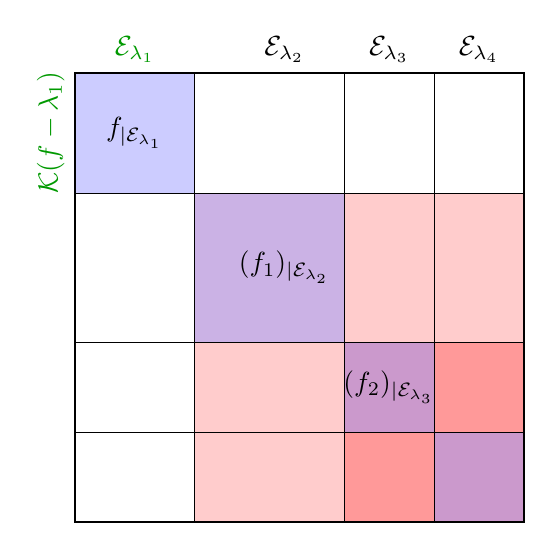
\begin{tikzpicture}[>=latex,thick,scale=0.38]
\uncover<2->{
\fill[color=blue!20] (0,11) rectangle (4,15);
\fill[color=red!20] (4,0) rectangle (15,11);
}
\uncover<3->{
\fill[color=red!40] (9,0) rectangle (15,6);
\fill[color=blue!40,opacity=0.5] (4,6) rectangle (9,11);
}
\uncover<4->{
\fill[color=blue!40,opacity=0.5] (9,3) rectangle (12,6);
\fill[color=blue!40,opacity=0.5] (12,0) rectangle (15,3);
}

\uncover<2->{
\draw[line width=0.1pt] (0,11) -- (15,11);
\draw[line width=0.1pt] (4,0) -- (4,15);
}

\uncover<3->{
\draw[line width=0.1pt] (0,6) -- (15,6);
\draw[line width=0.1pt] (9,0) -- (9,15);
}

\uncover<4->{
\draw[line width=0.1pt] (0,3) -- (15,3);
\draw[line width=0.1pt] (12,0) -- (12,15);
}
\draw (0,0) rectangle (15,15);
\uncover<2->{
\node[color=darkgreen] at (2,15) [above] {$\mathcal{E}_{\lambda_1}$};
\node[color=darkgreen] at (0,13) [above,rotate=90] {$\mathcal{K}(f-\lambda_1)$};
\node at (2,13) {$f_{|\mathcal{E}_{\lambda_1}}$};
}
\uncover<3->{
\node at (7,15) [above] {$\mathcal{E}_{\lambda_2}$};
\node at (7,8.5) {$(f_1)_{|\mathcal{E}_{\lambda_2}}$};
}
\uncover<4->{
\node at (10.5,15) [above] {$\mathcal{E}_{\lambda_3}$};
\node at (13.5,15) [above] {$\mathcal{E}_{\lambda_4}$};
\node at (10.5,4.5) {$(f_2)_{|\mathcal{E}_{\lambda_3}}$};
}
\end{tikzpicture}
\end{center}
\end{column}
\begin{column}{0.48\textwidth}
\begin{block}{Iteration}
$\Lambda=\{\lambda_1,\dots,\lambda_s\}$ Eigenwerte
\begin{align*}
\uncover<2->{
V
&=
\mathcal{K}(f-\lambda_1)
\oplus
\raisebox{-22pt}{\smash{\rlap{\tikz{\fill[color=red!20] (0,0) rectangle (1.83,1.1);}}}}
\underbrace{\mathcal{J}(f-\lambda_1)}_{\displaystyle=V_1}
}
\\[-15pt]
\uncover<2->{
f_1 &= f_{|V_1}
}
\\[10pt]
\uncover<3->{
V_1
&=
\mathcal{K}(f_1-\lambda_2)
\oplus
\raisebox{-22pt}{\smash{\rlap{\tikz{\fill[color=red!40] (0,0) rectangle (1.9,1.1);}}}}
\underbrace{\mathcal{J}(f_1-\lambda_2)}_{\displaystyle=V_2}
}
\\[-15pt]
\uncover<3->{
f_1 &= f_{|V_1}
}
\\
\uncover<4->{
&\phantom{0}\vdots
}
\end{align*}
\uncover<5->{%
$\Rightarrow$ $f$ hat {\color{blue}Blockdiagonalform} für die Zerlegung
\begin{align*}
V&=\bigoplus_{\lambda\in\Lambda} \mathcal{E}_{\lambda}
\end{align*}}
\end{block}
\end{column}
\end{columns}
\end{frame}
\egroup
